\chapter{Implementation}

This chapter provides a detailed explanation of our implementation strategy based on the outlined approach. The implemented solution consists of three core components: the Database, the RAGGIN core service, and the VS Code extension.

\section{Database}
\label{sec:Database}

\subsection{Data preparation}

The primary source of data for RAGGIN is the official documentation of the Next.js framework.

\begin{figure}[H]
	\centering
	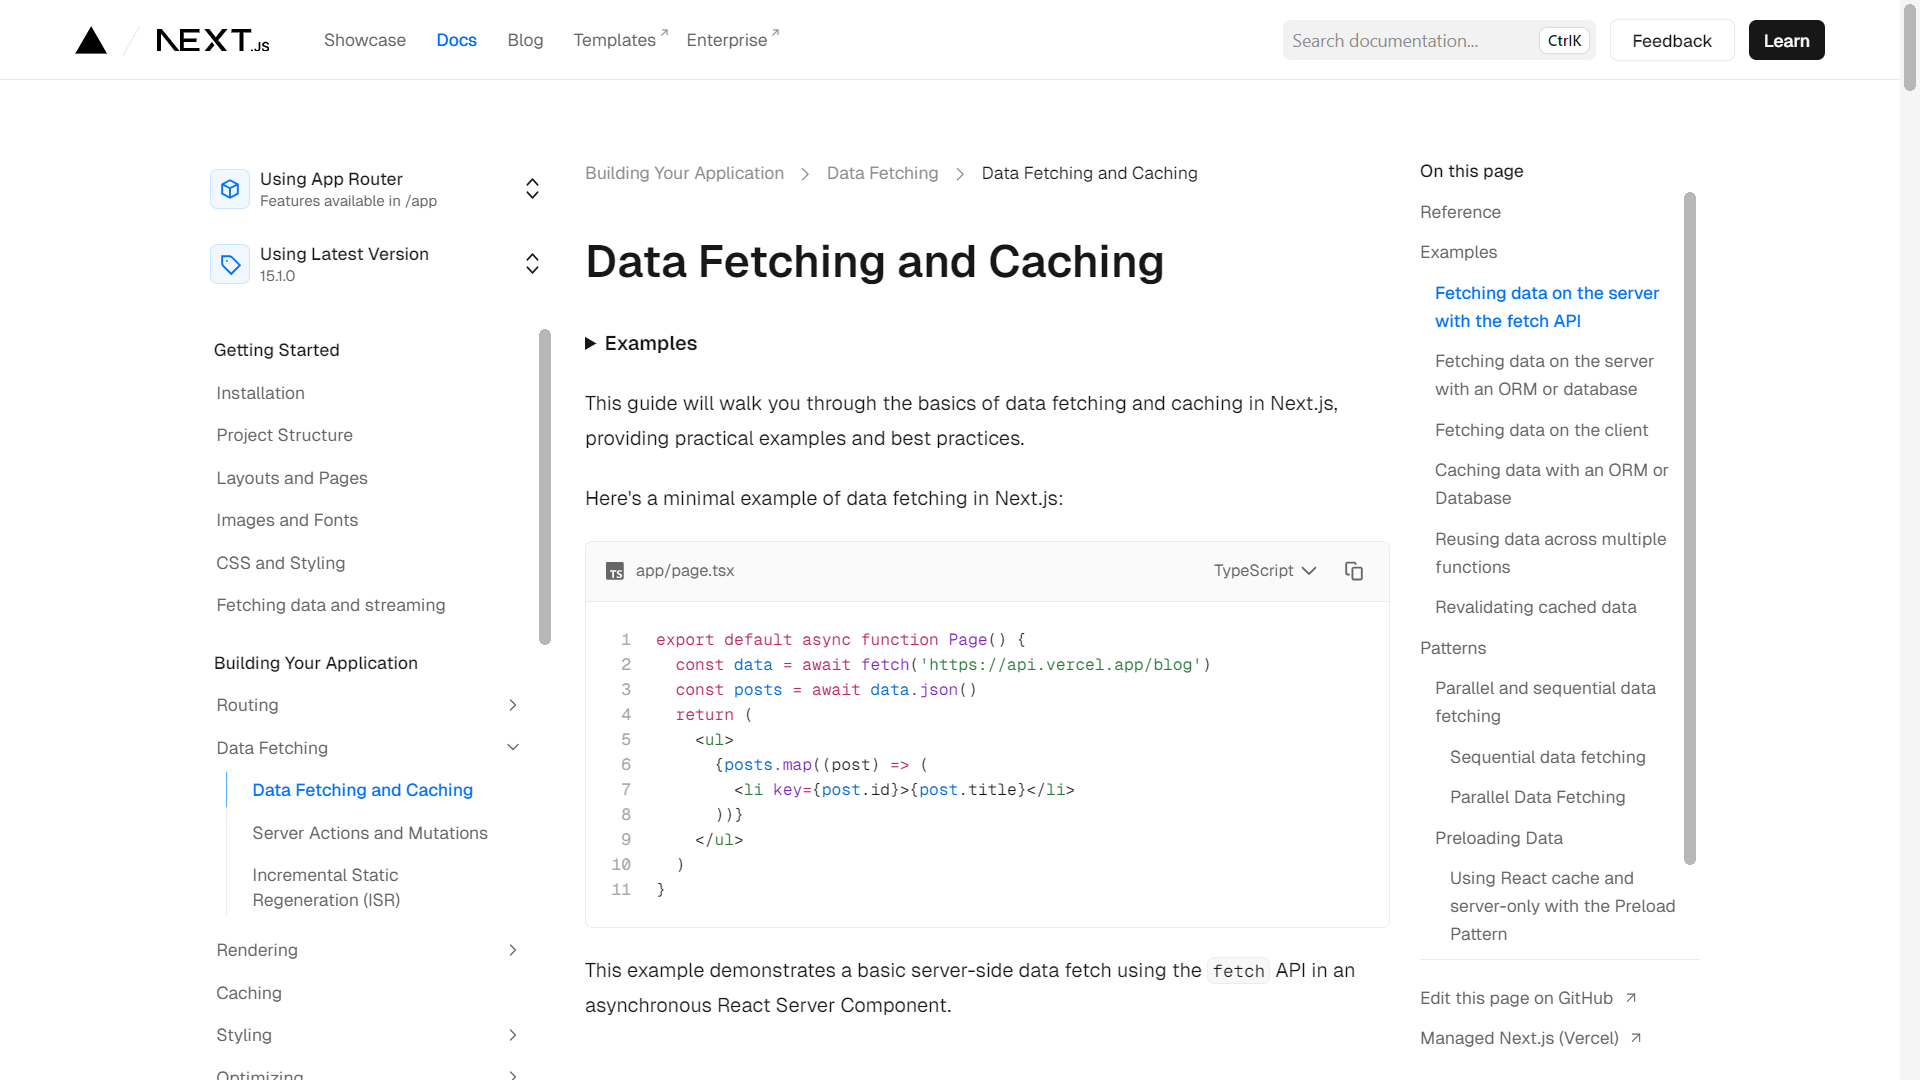
\includegraphics[width=1\textwidth]{Images/Approach/Documentation page example.png}
	\vspace{4mm}
	\caption{Example of a Next.js documentation page}
\end{figure}

\begin{figure}[H]
	\begin{Verbatim}[breaklines=true]
		
		---
		title: Data Fetching and Caching
		nav_title: Data Fetching and Caching
		description: Learn best practices for fetching data on the server or client in Next.js.
		---
		
		<details>
		<summary>Examples</summary>
		
		- [Next.js Commerce](https://vercel.com/templates/next.js/nextjs-commerce)
		- [On-Demand ISR](https://on-demand-isr.vercel.app)
		- [Next.js Forms](https://github.com/vercel/next.js/tree/canary/examples/next-forms)
		
		</details>
		
		This guide will walk you through the basics of data fetching and caching in Next.js, providing practical examples and best practices.
		
		Here's a minimal example of data fetching in Next.js:
		
		```tsx filename="app/page.tsx" switcher
		export default async function Page() {
			const data = await fetch('https://api.vercel.app/blog')
			const posts = await data.json()
			return (
			<ul>
			{posts.map((post) => (
				<li key={post.id}>{post.title}</li>
				))}
			</ul>
			)
		}
		```
		
		```jsx filename="app/page.js" switcher
		export default async function Page() {
			const data = await fetch('https://api.vercel.app/blog')
			const posts = await data.json()
			return (
			<ul>
			{posts.map((post) => (
				<li key={post.id}>{post.title}</li>
				))}
			</ul>
			)
		}
		```
		
		This example demonstrates a basic server-side data fetch using the `fetch` API in an asynchronous React Server Component.
	\end{Verbatim}
	\vspace{2mm}
	\captionof{figure}{Markdown representation of a documentation page}
\end{figure}

Upon reviewing the markdown files, we identified several main elements:

\begin{itemize}
	\item \textbf{Metadata.} Essential metadata includes:
	\begin{itemize}
		\item \texttt{title.} Title of the documentation page.
		\item \texttt{nav\_title}: Title displayed in the navigation bar.
		\item \texttt{description.} Concise summary of the content.
		\item \texttt{related.} Optional links to related documentation pages.
	\end{itemize}
	
	\item \textbf{Text content.} Main documentation content organized into sections and subsections via markdown syntax.
	
	\item \textbf{Code snippets.} Each snippet includes:
	\begin{itemize}
		\item \texttt{language.} Programming language (e.g., JavaScript or TypeScript).
		\item \texttt{file.} Corresponding filename or component name following Next.js conventions.
		\item \texttt{switcher.} Indicates if an alternative language snippet is available (e.g., JavaScript/TypeScript).
		\item \texttt{content.} Actual source code.
	\end{itemize}
	
	\item \textbf{Version history.} A dedicated section describing significant documentation updates across versions, although available in only a limited subset of documents.
\end{itemize}

We prepared documentation data for Next.js starting from version \texttt{v13.0.0} onwards. At the time of writing, the latest version is \texttt{v15.3.1}, encompassing a total of 107 supported versions. The data was sourced directly from the official Next.js GitHub repository.

\textbf{Steps involved in data preparation:}

\begin{itemize}
	\item \textbf{Data Acquisition.} A Python script leveraging Git's \texttt{sparse-checkout} feature was developed to efficiently download only relevant directories, such as \texttt{docs} and \texttt{errors}, corresponding to specific version tags. This script automates repository cloning, sparse-checkout configuration, and version-specific checkout.
	
	\item \textbf{Data Organization.} Retrieved files were systematically organized into directories structured by version. For example, documentation for version \texttt{v15.1.0} was organized as in Figure \ref{fig:v15dir}.
	
	\begin{figure}[H]
		\centering
		\begin{forest}
			for tree={
				font=\ttfamily,
				grow'=0,
				child anchor=west,
				parent anchor=south,
				anchor=west,
				calign=first,
				edge path={
					\noexpand\path [draw, \forestoption{edge}]
					(!u.south west) +(7.5pt,0) |- node[fill,inner sep=1.25pt] {} (.child anchor)\forestoption{edge label};
				},
				before typesetting nodes={
					if n=1
					{insert before={[,phantom]}}
					{}
				},
				fit=band,
				before computing xy={l=15pt},
			}
			[./v15.1.0/
			[docs/
			[01-app/]
			[index.mdx]
			[...]
			]
			[errors/
			[404-get-initial-props.mdx]
			[amp-bind-jsx-alt.mdx]
			[...]
			]
			]
		\end{forest}
		\vspace{5mm}
		\caption{Directory structure of retrieved documentation for version \texttt{v15.1.0}}
		\label{fig:v15dir}
	\end{figure}
	
\end{itemize}
	
After completing data preparation, the quantity of markdown files per version ranged significantly, from 294 files for \texttt{v13.0.0} to 591 files for \texttt{v15.3.1}. This increase nearly doubled the amount of documentation and documented errors, highlighting substantial growth in the capabilities and complexity of the Next.js framework.

\subsection{Data preprocessing}

After acquiring and organizing the data, the next critical step was preprocessing it to ensure alignment with our schema design for optimal storage and retrieval. This phase transformed raw markdown files into structured data via a Python-based preprocessing pipeline, leveraging markdown parsing libraries, embedding models, and structured data processing techniques.

\paragraph*{Key preprocessing steps}

\begin{itemize}
	\item \textbf{Metadata Extraction.}
	Metadata fields such as \texttt{title}, \texttt{description}, and \texttt{nav\_title} were extracted using the \texttt{frontmatter} library. Additional metadata, including \texttt{related} links when available, were also captured. Unique \texttt{entry\_id}s were generated for hierarchical referencing within the database schema.
	
	\begin{lstlisting}[language=Python, caption=Generating unique entry IDs]
		def generate_entry_id(file_path):
		relative_path = os.path.relpath(file_path)
		entry_id = re.sub(r'[^a-zA-Z0-9]', '_', relative_path)
		return entry_id.lower()
	\end{lstlisting}
	
	\item \textbf{Markdown parsing.} 
	Markdown files were parsed into components such as headings, paragraphs, lists, and code blocks using the \texttt{mistletoe} library. The root token, \texttt{Document}, represented the entire markdown file, while specific tokens such as \texttt{Heading}, \texttt{Paragraph}, and \texttt{List} enabled detailed content extraction while maintaining the document's hierarchy.
	
	\item \textbf{Content extraction.} 
	Each token's child elements were recursively processed to capture plain text, inline code, and hyperlinks. For example, \texttt{RawText} tokens represented basic text, \texttt{InlineCode} tokens identified inline code snippets, and \texttt{Link} tokens extracted hyperlink text and URLs.
	
	\item \textbf{Section segmentation.} 
	Logical sections were created based on \texttt{Heading} tokens in the markdown. Each section included a title, derived from the heading, and grouped content such as paragraphs, lists, or code blocks. This segmentation maintained the hierarchical structure necessary for efficient data retrieval.
	
	\item \textbf{Code snippet identification.} 
	Code blocks were identified using \texttt{CodeFence} tokens and extracted along with relevant metadata, including the programming language, associated filename, and optional switcher flags. This information linked code snippets to their respective sections and allowed for language-specific queries.
	
	\item \textbf{Embedding preparation.} 
	Text and code content from each section were processed to prepare for embedding generation. Sparse embeddings were used for keyword indexing, while dense embeddings captured semantic meaning, enabling similarity-based queries.
\end{itemize}

The \texttt{parse\_markdown\_sections} function, implemented using \texttt{mistletoe}, played a central role in these steps by iterating over the document tokens to extract structured information. For instance, a document with headings, paragraphs, and code blocks was transformed into hierarchical sections with associated metadata and content.

\begin{lstlisting}[language=Python, caption=Code snippet parsing]
	if isinstance(token, CodeFence):
	code_info = {
		"code": token.children[0].content if token.children else "",
		"language": token.language or "text",
		"filename": filename,
		"switcher": switcher
	}
\end{lstlisting}

\begin{itemize}
	\item \textbf{Embedding generation.} 
	Dense and sparse embeddings were generated for both text and code content using a pre-trained embedding model \texttt{BGEM3EmbeddingFunction}.
	
	\item \textbf{Storage.} 
	Processed entries were saved in batches as CSV files, with fields such as \texttt{entry\_id}, \texttt{text\_content}, and embeddings.
\end{itemize}

The preprocessing resulted in 107 CSV files, publicly accessible via our dataset \href{https://www.kaggle.com/datasets/jiyujizai/nextjs-documentation-for-raggin}{NextJs Documentation for RAGGIN}, achieving a usability score of 9.41/10 on Kaggle. Dataset insights include:

\begin{itemize}
	\item \textbf{Dataset size.} From 15.53 MB for version \texttt{v13.0.0} up to 49.97 MB for version \texttt{v15.3.1}.
	\item \textbf{Entry count.} Ranges from 396 entries for \texttt{v13.0.0} to 1,381 entries for \texttt{v15.3.1}.
\end{itemize}

\subsection{Database design}

Before presenting our schema design, we detail the properties utilized within our fields.

\begin{table}[H]
	\centering
	\label{tab:field_schema_properties}
	\begin{tabular}{p{3cm}p{5.5cm}p{5.5cm}l}
		\hline
		\textbf{Properties}   & \textbf{Description}                                                                 & \textbf{Note}                                                                                                                                         \\ \hline
		\texttt{name}         & Name of the field in the collection to create                                        & Data type: String. Mandatory                                                                                                                         \\ \hline
		\texttt{dtype}        & Data type of the field                                                              & Mandatory                                                                                                                                             \\ \hline
		\texttt{description}  & Description of the field                                                            & Data type: String. Optional                                                                                                                          \\ \hline
		\texttt{is\_primary}  & Whether to set the field as the primary key field or not                            & Data type: Boolean. Mandatory for the primary key field                                                            \\ \hline
		\texttt{auto\_id}     & Switch to enable or disable automatic ID (primary key) allocation                   & Data type: Boolean. Mandatory for primary key field                                                                                     \\ \hline
		\texttt{max\_length}  & Maximum byte length for strings allowed to be inserted.                             & {[}1, 65,535{]}. Mandatory for \texttt{VARCHAR} field. byte                                            \\ \hline
		\texttt{dim}          & Dimension of the vector                                                            & Data type: Integer {[}1, 32,768{]}. Mandatory for dense vector field. Omit for sparse vector field                                                   \\ \hline
		\texttt{is\_partition\_key} & Whether this field is a partition-key field                                      & Data type: Boolean                                                                                           \\ \hline
	\end{tabular}
	\caption{Field schema properties\protect\footnotemark}
\end{table}

\footnotetext{Manage Schema - \url{https://milvus.io/docs/schema.md\#Manage-Schema}}

We developed a schema optimized for organizing and storing documentation data. The schema is implemented within a single collection named \texttt{nextjs\_docs}.

\begin{table}[H]
	\small
	\centering
	\setlength\tabcolsep{5pt}
	\renewcommand{\arraystretch}{1.2}
	\begin{tabular}{l c c p{6.8cm}}
		\hline
		\textbf{Field} & \textbf{dtype} & \textbf{Len / Dim} & \textbf{Notes  /  Description} \\ \hline
		\texttt{entry\_id}           & VARCHAR                & 255  & \textbf{Primary key}. auto\_id\,=\,false.  Built by concatenating version + doc name + section name.\\
		\texttt{title}               & VARCHAR                & 255  & Built from documentation name, description, and section name.\\
		\texttt{metadata}            & JSON                   & –    & JSON blob of title, description, and related links.\\
		\texttt{version}             & VARCHAR                & 20   & \textbf{Partition key}.  Indicates documentation version.\\
		\texttt{tag}                 & VARCHAR                & 255  & Labels source (documentation vs.\ documented errors).\\
		\hline
		\texttt{text\_content}       & VARCHAR                & 65\,535 & Markdown body.\\
		\texttt{code\_content}       & VARCHAR                & 65\,535 & JSON-stringified dict of code snippets \\
		\hline
		\texttt{sparse\_title}       & SPARSE\_FLOAT\_VECTOR  & –    & Sparse embedding of concatenated title + description.  \emph{Index}: SPARSE\_INVERTED\_INDEX; \emph{Metric}: Inner Product.\\
		\texttt{dense\_text\_content}& FLOAT\_VECTOR          & 1024 & Dense embedding of full text.  \emph{Index}: HNSW; \emph{Metric}: Cosine.\\
		\texttt{dense\_code\_snippet}& FLOAT\_VECTOR          & 1024 & Avg-pooled vector over all snippet embeddings.  \emph{Index}: HNSW; \emph{Metric}: Cosine.\\
		\hline
	\end{tabular}
	\caption{Schema structure}
	\label{tab:schema_structure}
\end{table}

When designing the schema, it is crucial to determine how to store code snippets effectively while facilitating the identification of which snippet belongs to which section. Our proposal is to avoid saving code snippets as separate entries in the database in order to reduce latency and computational overhead.

Given this decision, a challenge arises. How should we store embeddings of code snippets, especially since some sections contain none, one, or multiple code snippets? Additionally, for sections with multiple snippets, we must define an efficient storage method.

Figure~\ref{fig:code_snippet_distribution} illustrates the distribution of code snippets across sections from version \texttt{v15.1.4} to \texttt{v15.3.1}. It shows that while some sections have multiple snippets, others have none, reinforcing the need for a flexible storage strategy.

\begin{figure}[H]
	\centering
	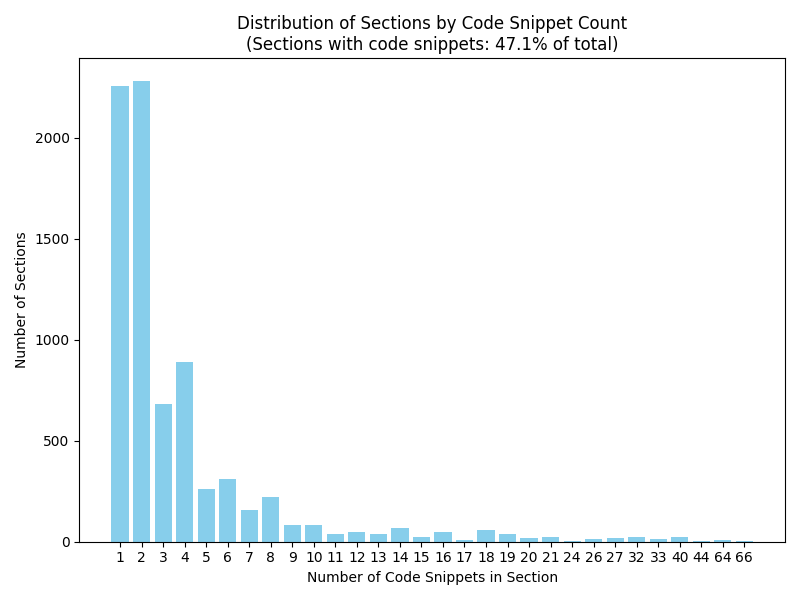
\includegraphics[width=0.9\textwidth]{Images/Implement/section_code_snippet_count_distribution.png}
	\vspace{3mm}
	\caption{Distribution of Code Snippets per Section (\texttt{v15.1.4} to \texttt{v15.3.1})}
	\label{fig:code_snippet_distribution}
\end{figure}

\begin{figure}[H]
	\centering
	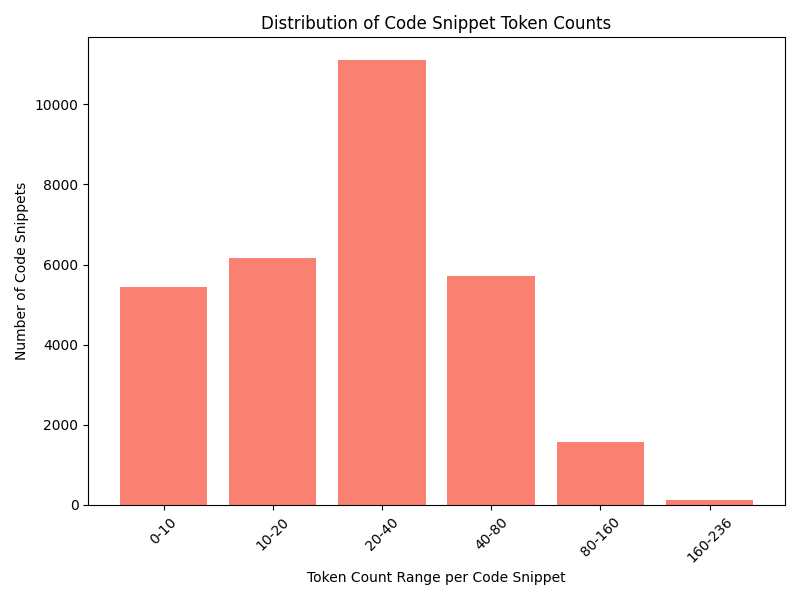
\includegraphics[width=0.9\textwidth]{Images/Implement/code_snippet_token_count_distribution.png}
	\vspace{3mm}
	\caption{Token Count Distribution of Code Snippets (\texttt{v15.1.4} to \texttt{v15.3.1})}
	\label{fig:code_snippet_token}
\end{figure}

There are two primary methods for embedding code snippets:
\begin{itemize}
	\item \textbf{Separate storage.} Each code snippet embedding is stored individually within an array field associated with its section entry.
	\item \textbf{Aggregated storage.} Embeddings of all code snippets within a section are aggregated into a single vector.
\end{itemize}

The separate storage method enables precise comparison between a query and individual code snippets. However, it suffers from major drawbacks:
\begin{itemize}
	\item Additional complexity in indexing entries, as the number of code snippets per section varies.
	\item Increased database size and computational cost, particularly problematic for large-scale retrieval tasks.
\end{itemize}

Thus, aggregated storage is the preferred option for efficiency.

To unify embeddings into a single vector per section, two aggregation methods are considered:
\begin{itemize}
	\item \textbf{Average pooling.} Element-wise averaging of all embeddings.
	\item \textbf{Max pooling.} Element-wise maximum of all embeddings.
\end{itemize}

To evaluate which aggregation method performs better, we utilize Normalized Discounted Cumulative Gain (NDCG) as the ranking metric.

\[
\text{DCG}(s) = \sum_{i=1}^{n} \frac{2^{s_i} - 1}{\log_2(i + 1)}, \quad
\text{NDCG}(s) = \frac{\text{DCG}(s)}{\text{DCG}(s^{\ast})}
\]

where \( s = [s_1, s_2, \ldots, s_n] \) is the list of relevance scores, and \( s^{\ast} \) is the ideal ranking of the same elements sorted in descending order by relevance.

Figures~\ref{fig:ndcg_avg} and~\ref{fig:ndcg_max} present the NDCG performance of average pooling and max pooling, respectively, evaluated under both dense code search and hybrid search scenarios.

\begin{figure}[H]
	\centering
	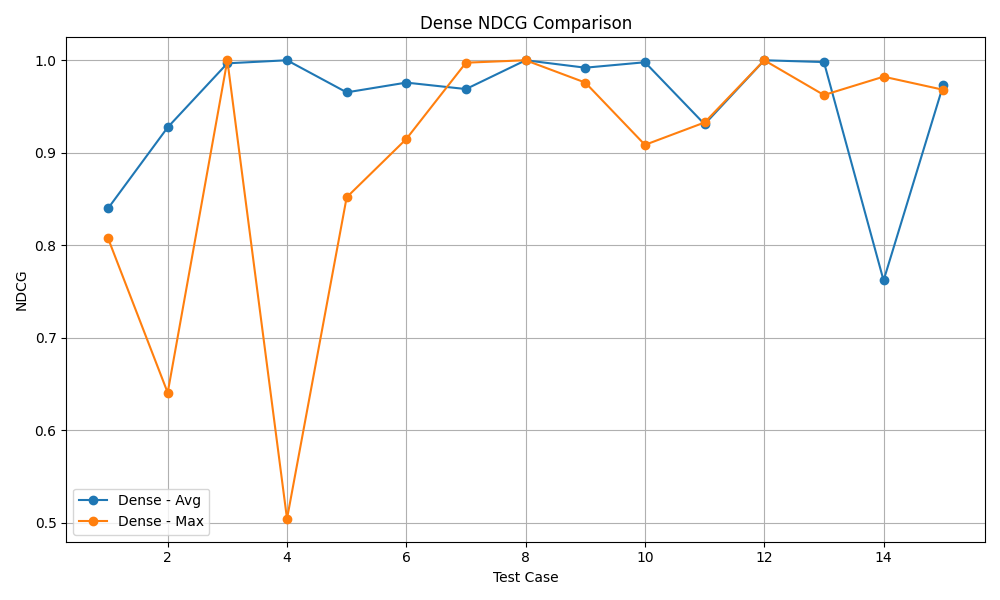
\includegraphics[width=0.9\textwidth]{Images/Implement/dense_code_ndcg.png}
	\vspace{5mm}
	\caption{NDCG results with dense code search}
	\label{fig:ndcg_avg}
\end{figure}

\begin{figure}[H]
	\centering
	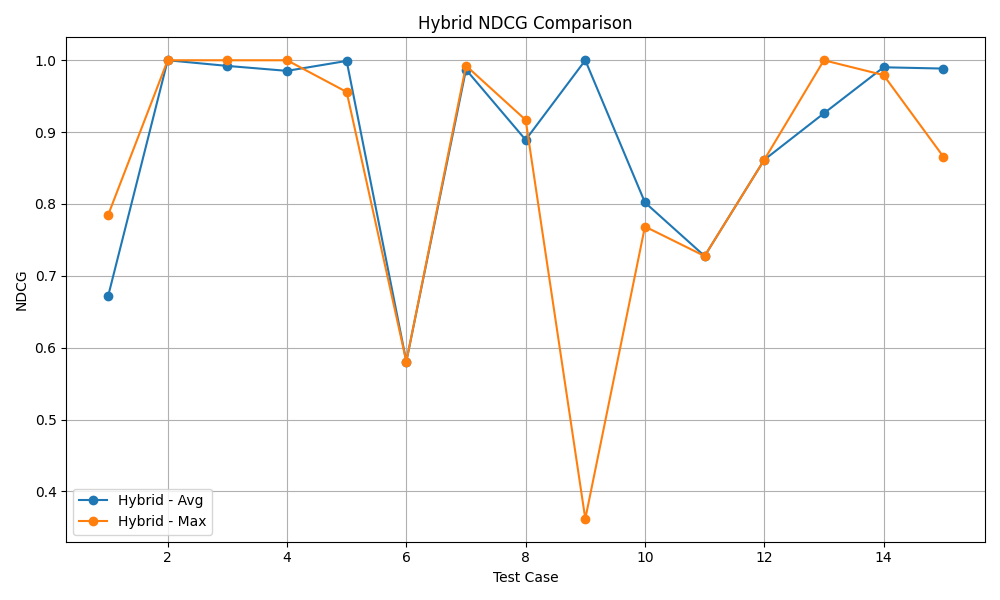
\includegraphics[width=0.9\textwidth]{Images/Implement/hybrid_ndcg.png}
	\vspace{5mm}
	\caption{NDCG results with hybrid search}
	\label{fig:ndcg_max}
\end{figure}

The evaluation results indicate that average pooling delivers more stable and reliable retrieval performance than max pooling, particularly in maintaining consistent ranking quality.

The retrieved document structure includes a text body containing special placeholder tokens in the form of \texttt{code\_snippet\_\{idx\}}. During post-processing, each placeholder is replaced by the corresponding code snippet from the \texttt{code\_content} dictionary.

\subsection{Database setup}

To efficiently handle storage, retrieval, and indexing, we set up our database using Milvus, leveraging Docker Compose for streamlined deployment and configuration. This database setup involved three key services:

\begin{itemize}
	\item \textbf{etcd service.}
	We utilized the \texttt{etcd} container to manage metadata storage and configuration. It uses the CoreOS etcd image version \texttt{v3.5.16}. Configuration settings included client URL advertisement, client listening URLs, data directory specification, auto-compaction, and backend quota management to ensure efficient and stable operation.
	
	\item \textbf{MinIO service.}
	The \texttt{minio} container was configured for object storage, essential for storing large data objects. The MinIO server uses a specific release version and provides object storage capabilities with secure access via defined credentials. It exposes two ports: one for the main service (port \texttt{9000}) and another for the console interface (port \texttt{9001}).
	
	\item \textbf{Milvus service.}
	The \texttt{milvus-standalone} service, using Milvus version \texttt{v2.5.4}, was established for vector indexing and retrieval operations. This container depends on the healthy states of both \texttt{etcd} and \texttt{minio} services, integrating with them via their respective endpoints. It handles incoming requests and provides monitoring via specified ports.
\end{itemize}

\subsection{Database API}

The Database API manages documentation data in the Milvus database through seven primary endpoints:

\begin{itemize}
	
	\item \textbf{List all supported versions} \texttt{[GET /data/versions].}  
	Returns a list of all supported Next.js versions with download status.
	\begin{lstlisting}[caption=GET /data/versions output example]
		[
		{"version_name": "v13.0.0", "downloaded": true},
		{"version_name": "v13.0.1", "downloaded": false},
		...
		{"version_name": "v15.3.1", "downloaded": true}
		]\end{lstlisting}
	
	\item \textbf{Retrieve version details} \texttt{[GET /data/versions/\{version\}].}  
	Fetches metadata (file size, last modified time) for a specific version. Returns 404 if unsupported.
	\begin{lstlisting}[caption=GET /data/versions/{version} output example]
		{
			"version_name": "v15.3.1",
			"downloaded": true,
			"file_size": 49966271,
			"last_modified": 1745841921.8775475
		]\end{lstlisting}
	
	\item \textbf{List downloaded versions} \texttt{[GET /data/downloaded].}
	Returns a list of all versions downloaded locally.
	\begin{lstlisting}[caption=GET /data/downloaded output example]
		[
		"v13.0.0",
		"v15.1.2",
		"v15.3.1"
		]\end{lstlisting}
	
	\item \textbf{Retrieve version statistics} \texttt{[GET /data/stats].}  
	Provides statistics including total supported and downloaded versions.
	\begin{lstlisting}[caption=GET /data/stats output example]
		{
			"total_supported": 107,
			"total_downloaded": 3,
			"downloaded_versions": [
			"v13.0.0",
			"v15.1.2",
			"v15.3.1"
			]
		}\end{lstlisting}
	
	\item \textbf{Retrieve documentation version} \texttt{[POST /version/retrieve].} 
	Downloads a version from Kaggle (if absent) and inserts it into Milvus with optional indexing parameters.
	
	Request parameters:
	\begin{itemize}
		\item \texttt{version\_name.} Target version (e.g., \texttt{v15.0.0}).
		\item \texttt{m\_text} (optional, default = 16). HNSW \texttt{M} for text embeddings.
		\item \texttt{ef\_text} (optional, default = 200). HNSW \texttt{efConstruction} for text embeddings.
		\item \texttt{m\_code} (optional, default = 16). HNSW \texttt{M} for code embeddings.
		\item \texttt{ef\_code} (optional, default = 200). HNSW \texttt{efConstruction} for code embeddings.
	\end{itemize}
	
	Processing steps:
	\begin{enumerate}
		\item Check if CSV exists locally.
		\item Download CSV from Kaggle if missing.
		\item Create Milvus collection if not exists; apply index parameters (\texttt{M}, \texttt{efConstruction}) specific to the version. 
		\begin{itemize}
			\item \texttt{M}: Controls graph connectivity in HNSW; higher values improve accuracy but use more memory.
			\item \texttt{efConstruction}: Controls the candidate pool size during indexing; larger values increase precision at indexing cost.
		\end{itemize}
		\item Insert parsed CSV data into Milvus.
	\end{enumerate}


	\item \textbf{Repair documentation version} \texttt{[POST /version/repair]}:  
	Repairs a version by deleting old data and reimporting it.
	
	Request parameters:
	\begin{itemize}
		\item \texttt{version\_name}. Target version.
		\item Optional indexing parameters (\texttt{m\_text}, \texttt{ef\_text}, \texttt{m\_code}, \texttt{ef\_code}).
	\end{itemize}
	
	Processing steps:
	\begin{enumerate}
		\item Remove local CSV and associated Milvus entries.
		\item Download fresh CSV from Kaggle.
		\item Recreate Milvus indices using specified or default \texttt{M} and \texttt{efConstruction} values.
		\item Reinsert data into Milvus.
	\end{enumerate}


	\item \textbf{Delete documentation version} \texttt{[DELETE /version/delete]}:  
	Deletes a version from both local storage and Milvus.
	
	Request parameters:
	\begin{itemize}
		\item \texttt{version\_name}: Target version.
	\end{itemize}
	
	Processing steps:
	\begin{enumerate}
		\item Check if CSV exists locally.
		\item Remove associated entries from Milvus.
		\item Delete the local CSV file.
	\end{enumerate}
	
\end{itemize}

\section{RAGGIN core services}
\label{sec:raggin-core}

The RAGGIN core service provides the API functionalities for hybrid retrieval and generation. It is deployed as a containerized application, built from a custom Dockerfile and exposed through port \texttt{8000}. The backend interacts directly with the Milvus vector database via a specified internal URI, handling retrieval queries and database operations. It also interfaces with an external Ollama API endpoint to access local LLMs during generation. Pretrained embedding models are cached within a dedicated volume to reduce startup latency and accelerate embedding generation. The backend depends on the Milvus standalone service for healthy initialization, ensuring database availability before serving requests. Volumes are mounted to persist downloaded documentation files and model checkpoints across restarts, allowing efficient reuse of data. This service acts as the main processing layer connecting the vector storage, retrieval logic, and language model inference.

\subsection{Retriever}

The Retriever service performs hybrid searches by combining sparse lexical matching and dense vector similarity using BGE-M3 \cite{chen2024bge} embeddings. It leverages Milvus for efficient retrieval and supports weighted multi-modal queries.

\paragraph*{Hybrid search endpoint \texttt{[POST /search]}}

Executes hybrid searches across sparse and dense (text and code) embeddings, returning the top-\textit{K} most relevant results.

Request parameters:

\begin{itemize}
	\item \texttt{text\_query.} Text query for semantic matching.
	\item \texttt{code\_query.} Code query for snippet matching.
	\item \texttt{version\_name.} Version filter (e.g., \texttt{v15.0.0}).
	\item \texttt{sparse\_weight} (optional, default = 1.0). Weight for sparse embeddings.
	\item \texttt{dense\_text\_weight} (optional, default = 1.0). Weight for dense text embeddings.
	\item \texttt{dense\_code\_weight} (optional, default = 1.0). Weight for dense code embeddings.
	\item \texttt{top\_k} (optional, default = 5). Number of results to return.
	\item \texttt{filter\_expr} (optional). Additional filter expression\footnote{Filtered Search - \url{https://milvus.io/docs/filtered-search.md}} for Milvus.
	\item \texttt{radius\_sparse}, \texttt{radius\_dense\_text}, \texttt{radius\_dense\_code} (optional, default = 0.5). Search radius\footnote{Range Search - \url{https://milvus.io/docs/range-search.md}} for each modality.
   	\item \texttt{range\_sparse}, \texttt{range\_dense\_text}, \texttt{range\_dense\_code} (optional, default = 0.5). Search range\footnote{Range Search - \url{https://milvus.io/docs/range-search.md}} for each modality.
\end{itemize}

Processing steps:

\begin{enumerate}
	\item \textbf{Validate input.} Ensure at least one modality weight is nonzero; prepare queries and filters.
	\item \textbf{Generate embeddings.} Produce sparse and dense vectors using BGE-M3 \cite{chen2024bge}.
	\item \textbf{Search.} Query Milvus separately for each modality (sparse, dense text, dense code).
	\item \textbf{Merge results.} Raw similarity distances returned by Milvus are mapped to the range \([0, 1]\) to ensure comparability across modalities.  
	The normalization function is defined as:
	
	\[
	\text{normalized\_score} = \frac{\frac{\pi}{2} - \arctan(\text{distance})}{\frac{\pi}{2}}
	\]
	
	where:
	\begin{itemize}
		\item A distance close to 0 maps to a score close to 1 (indicating high relevance).
		\item A distance approaching \(+\infty\) maps to a score close to 0 (indicating low relevance).
		\item The output is clamped to \([0, 1]\) to avoid overflow or underflow.
	\end{itemize}
	
	This mapping ensures that smaller distances (closer matches) correspond to higher normalized scores.
	
	After normalization, scores from different modalities (sparse, dense text, dense code) are aggregated into a single combined score using a weighted sum:
	
	\[
	\text{combined\_score} = w_{\text{sparse}} \times s_{\text{sparse}} + w_{\text{dense\_text}} \times s_{\text{dense\_text}} + w_{\text{dense\_code}} \times s_{\text{dense\_code}}
	\]
	
	where:
	\begin{itemize}
		\item \(w_{\text{sparse}}, w_{\text{dense\_text}}, w_{\text{dense\_code}}\) are the user-defined weights for each modality.
		\item \(s_{\text{sparse}}, s_{\text{dense\_text}}, s_{\text{dense\_code}}\) are the normalized scores from the respective search results.
	\end{itemize}
	
	\item Select top-\textit{K} rank by hybrid scores and return top results.
\end{enumerate}

Example query:

\begin{lstlisting}[caption=POST /search JSON payload example]
	{
		"text_query": "Is this command using the canary version?",
		"code_query": "npx create-next-app@latest",
		"version_name": "v15.1.2",
		"sparse_weight": 0.5,
		"dense_text_weight": 1.0,
		"dense_code_weight": 0.9,
		"top_k": 3,
		"filter_expr": "tag == 'documentation'",
		"radius_sparse": 0.08,
		"range_sparse": 1,
		"radius_dense_text": 0.6,
		"range_dense_text": 1,
		"radius_dense_code": 0.6,
		"range_dense_code": 1
	}
\end{lstlisting}

Example response:

\begin{lstlisting}[caption=POST /search output example]
	{
		"results": [
		{
			"title": "02-canary - Upgrade your Next.js Application to canary",
			"metadata": {},
			"version": "v15.3.1",
			"text_content": "...",
			"code_content": "...",
			"tag": "documentation",
			"sparse_distance": 0.115,
			"dense_text_distance": 0.602,
			"dense_code_distance": null,
			"combined_score": 0.745
		},
		{
			"title": "create-next-app - Create Next.js apps",
			"metadata": {},
			"version": "v15.3.1",
			"text_content": "...",
			"code_content": "...",
			"sparse_distance": 0.080,
			"dense_code_distance": 0.901,
			"combined_score": 0.681
		},
		{
			"title": "12-upgrading - Learn how to upgrade Next.js",
			"metadata": {},
			"version": "v15.3.1",
			"text_content": "...",
			"code_content": "...",
			"dense_text_distance": 0.664,
			"combined_score": 0.626
		}
		]
	}
\end{lstlisting}

\subsection{Generator}

\paragraph*{Local LLMs setup.} In the development of RAGGIN, the choice of a robust and secure LLM is critical for achieving high-quality responses and ensuring data privacy. To support our RAG pipeline, we installed and configured Ollama\footnote{Ollama - \url{https://ollama.com/}}, a platform specifically designed to facilitate the deployment of pre-trained language models on local infrastructure. This section describes the setup and integration of Ollama into our system.

\paragraph*{Setup Ollama.} The setup process begins by installing the Ollama application, which is compatible with various operating systems including Windows, macOS, and Linux. Once installed, Ollama provides a straightforward interface to download and configure pre-trained models without requiring fine-tuning.

The installation of specific models is conducted via the command prompt or terminal, with available models conveniently listed on \url{https://ollama.com/search}.
The command to install a model is \verb|ollama pull <model_name>|.

Once a model is installed, it is stored locally, ensuring a high level of data privacy and security - an essential feature for applications dealing with sensitive or proprietary information. To test the model, we can use the command \verb|ollama run <model_name>| .

Furthermore, the platform's lightweight design enhances compatibility across a variety of hardware configurations, making it particularly suitable for environments with limited computational resources. This flexibility makes Ollama an optimal choice for deploying local LLMs in diverse use cases.

% For instance, installing a model such as Meta's llama3.2  can be accomplished with the following command:

% \begin{verbatim}
	% ollama pull llama3.2
	% \end{verbatim}



% This command downloads the desired model and sets up the necessary configurations, enabling immediate usage. Ollama’s design ensures that users do not need to worry about manual configurations, as the system handles all dependencies and environment settings.




\paragraph*{Integration with RAGGIN.} To integrate Ollama into the RAG workflow, we use the Ollama API for direct interaction with the locally installed models. The endpoint for the API is:

POST \url{http://localhost:11434/api/generate}

The POST request body should be in JSON format, specifying the desired model and the prompt to be processed.

\begin{lstlisting}[caption=Ollama JSON payload example]
	{
		"model": "qwen",
		"prompt": "What is RAG?"
	}
\end{lstlisting}

The API provides a straightforward and efficient method for passing queries and receiving responses from the model. 

%Alternatively, Ollama models can also be integrated using the Python library LangChain\footnote{LangChain - \url{https://python.langchain.com/docs/introduction/}}. With LangChain, the locally installed Ollama models can be accessed and utilized as part of a more comprehensive pipeline, allowing for advanced customization and ease of interaction. This flexibility enables developers to build robust RAG systems that leverage the full potential of Ollama's capabilities while adapting to diverse use cases.


\textbf{Generator endpoint \texttt{[POST /prompt/generate]}}

When RAGGIN Generator receives the generate request, it will take the query, model, and file list and process them to RAGGIN Retriever to retrieve relevant documents. Then, it will take the retrieved documents, together with the query and process them to Ollama LLM to generate the final response.

Request parameters:
\begin{itemize}
	\item \texttt{version\_name.} Version filter (e.g. \texttt{v15.3.1}).
	\item \texttt{query.}: The input query or prompt that serves as the basis for the system to retrieve relevant information and generate a response.
	\item \texttt{model.}: The name of the Ollama LLM selected for generating the response.
	\item \texttt{file\_list} (optional). A collection of \texttt{FileModel} instances, where each instance includes the following string fields: \texttt{fileName}, \texttt{fileExtension}, and \texttt{fileContent}.
	\item \texttt{additional\_options} (optional). An optional field comprising two subfields: \texttt{retriever\_options}, the configurable parameters associated with the hybrid search endpoint and \texttt{generator\_options} - the set of options controlling the language model's generation behavior.
	
\end{itemize}

Processing steps:

\begin{enumerate}
	\item \textbf{Retrieve documents.} Use input prompt and version name to retrieve relevance documents.
	\item \textbf{Enhance prompt.} Construct an enhanced prompt using the original prompt with the retrieved documents.
	\item \textbf{Generate.} Send a POST request to the Ollama API endpoint, then receive and return the generated response.

\end{enumerate}

The generate request's body should be in JSON format, specifying the desired model and the prompt to be processed.

\begin{lstlisting}[caption=POST /prompt/generate JSON payload example]
{
    "version_name": "v15.1.3",
    "query": "refactor the files to make it more readable.",
    "model": "llama2:13b",
    "additional_options": {
        "retriever_options": {
        	"top_k": 5
        },
        "generator_options": {
        	"temperature": 0.8
        }
    },
    "file_list": [
        {
        "file_name": "/my_page.tsx",
        "file_extension": "tsx",
        "file_content": "import { File, UserRound, LogOut } from \"lucide-react\"; ..."
        }
    ]
}
\end{lstlisting}

The response body will contain the generated response and some other relevant information in JSON format.

\begin{lstlisting}[caption=POST /prompt/generate output example]
{
    "model": "llama2:13b",
    "response": "Sure! Here are some suggestions for refactoring the code to make it more 
    readable ..."
    ...
}
\end{lstlisting}


\section{VS Code Extension}
\label{sec:VS Code Extension}
The VS Code extension, also named RAGGIN, serves as an interface between the user and a locally hosted execution core running in Docker. After the user downloads the RAGGIN core (see Section~\ref{sec:raggin-core}), they can interact with it directly through the extension’s built-in UI in VS Code. A detailed description of the user interface is provided in Appendix~\ref{appendix:interface}.

\subsection{Intialize RAGGIN codebase}
The setup process for the RAGGIN VS Code extension follows the standard procedures outlined in the official VS Code extension development documentation\footnote{Your first extension - \url{https://code.visualstudio.com/api/get-started/your-first-extension}}.


Our initial codebase followed the directory structure illustrated below. It primarily consists of two main folders: \texttt{src} and \texttt{webview-ui}.

\begin{itemize}
	\item \texttt{src.} This directory serves as the extension layer, responsible for implementing the core functionalities, including API calls to the RAGGIN core or a local Ollama server. It also manages the integration with VSCode's webview API to render content dynamically.
	
	\item \texttt{webview-ui.} This folder handles the complete UI implementation displayed within the VSCode sidebar, providing a seamless and interactive user experience.
\end{itemize}
\begin{figure}[H]
	\centering 
	\begin{forest}
		for tree={
			font=\ttfamily,
			grow'=0,
			child anchor=west,
			parent anchor=south,
			anchor=west,
			calign=first,
			edge path={
				\noexpand\path [draw, \forestoption{edge}]
				(!u.south west) +(7.5pt,0) |- node[fill,inner sep=1.25pt] {} (.child anchor)\forestoption{edge label};
			},
			before typesetting nodes={
				if n=1
				{insert before={[,phantom]}}
				{}
			},
			fit=band,
			before computing xy={l=15pt},
		}
		[system
			[.vscode // Config for launching and debugging the extension
				[launch.json // Config for launching and debugging the extension]
				[task.json  // Config for build task that compiles TypeScript]
			] 
			[media // Store icons for RAGGIN] 
			[src // Extension layer source code] 
			[webview-ui // UI source code] 
			[package.json // Extension manifest] 
			[tsconfig.json  // TypeScript configuration]
		]
	\end{forest}
	\vspace{5mm}
  \caption{RAGGIN codebase directory tree}
  \label{fig:tree}
\end{figure}

\subsection{VS Code extension webview comunication}
VS Code provides a post-message communication mechanism that enables interaction between the extension backend and the webview. This system is particularly useful for initiating processes, requesting data, or triggering UI updates. To facilitate this communication, both the extension layer and the webview can send messages and listen for incoming ones, ensuring a seamless two-way data exchange.
\begin{figure}[H]
	\centering
		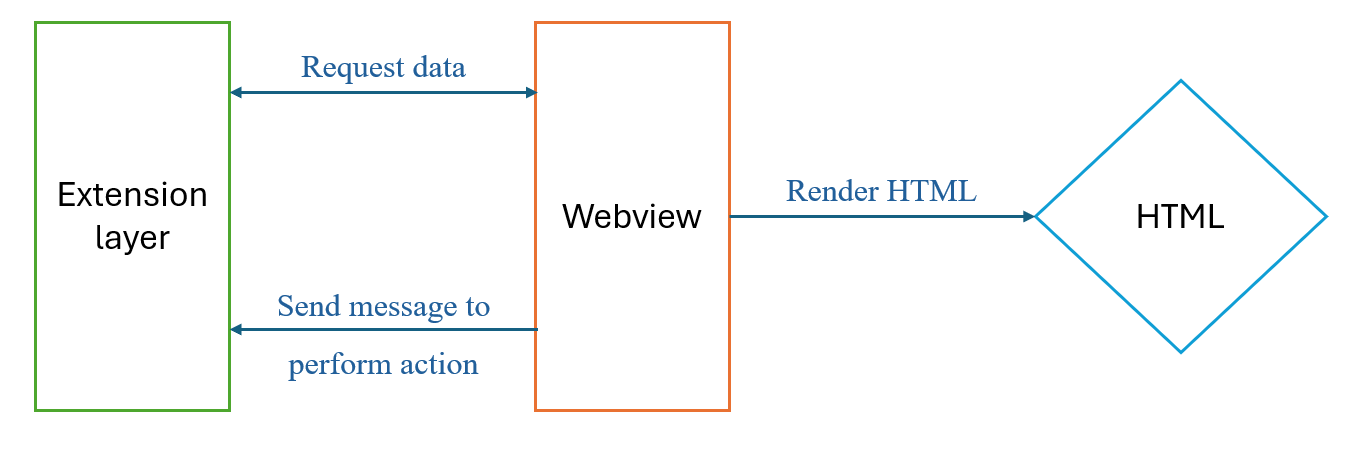
\includegraphics[width=0.9\textwidth]{Images/Implement/webview_communication.png}
	\vspace{3mm}
	\caption{API like communication flow}
	\label{fig:webview_communication}
\end{figure}

\paragraph*{Rendering RAGGIN UI in VS Code.} In the development of VS Code extensions, presenting a custom UI that aligns with the extension's functionality is often necessary. While VS Code provides native APIs for UI components, there are scenarios where these APIs are insufficient for complex or highly customized interfaces. In such cases, the webview API offers a powerful solution, enabling the integration of custom HTML, CSS, and JavaScript-based UIs within the extension environment.

The Webview API allows developers to embed fully customized front-end applications within VS Code, enabling the use of modern frameworks such as React\footnote{React - \url{https://react.dev/}}. This approach greatly streamlines the development of complex interfaces by supporting dynamic rendering, component reuse, and efficient state management. Using React within a Webview context provides benefits such as a modular component structure, performance gains through the virtual Document Object Model (DOM), and access to a wide range of supporting libraries-ultimately leading to faster development and easier long-term maintenance.

For icon rendering in the extension UI, we chose the codicon\footnote{codicon - \url{https://microsoft.github.io/vscode-codicons/dist/codicon.html}} library over other popular options such as react-icons or lucide-icons. This decision was made because, within the webview environment which is a sandboxed HTML container in VS Code-libraries like React-based icons or modern Scalable Vector Graphics (SVG) icon sets often fail to render correctly due to DOM restrictions and complex bundling requirements. Also, codicon is the official icon set used internally by VS Code and is natively supported within webview environments without the need for external imports

To make the user interface more polished and the development process smoother, we chose to use the Shadcn UI library\footnote{Shadcn UI - \url{https://ui.shadcn.com/}}. It's a modern set of accessible, unstyled components built on Radix UI, designed specifically for React projects. With ready-to-use elements like buttons, tooltips, modals, and popover, it helps us keep a consistent design throughout the RAGGIN extension, while also saving time that would otherwise be spent styling each component from scratch.

\paragraph*{Establish Communication.} To establish communication between the webview and the extension backend, VS Code provides a structured messaging system based on the \texttt{postMessage} API. This mechanism enables asynchronous, bidirectional communication where serialized messages, typically JSON objects are exchanged between the frontend and backend. On the webview side, messages are sent using the VS Code API, while the extension receives and handles them through registered event listeners. Conversely, the extension can respond by sending messages back to the webview, which listens using standard browser events. This design enables interactions such as form submissions, real-time updates, and API calls. 

In the specific context of RAGGIN, when the user enters a prompt and presses the send button on the UI, the webview API is used to transmit the request to the extension.
\begin{lstlisting}[caption=Handle chat storing]
const vscode = acquireVsCodeApi();
vscode.postMessage({
	command: "ragCall",
	// Parameters transmit
	...
});
\end{lstlisting}

When the extension layer receives the \texttt{ragCall} command, it validates required parameters, call API in the RAGGIN core to take the response. The extension layer then sends a message back to the webview.

\begin{lstlisting}[caption=Extension layer receives command from webview]
case "ragCall": {
	// Validate parameters
	...	
	try {
		webviewView.webview.postMessage({
			command: "ragCallComplete",
			content: answer.response,
			...
		});
	} catch (error) {
		// Handling errors
		...
	}
	break;
}
\end{lstlisting}

Finally, the webview has an event listener that detects the \texttt{ragCallComplete} message and then store the response in history and render it to chat window.

\begin{lstlisting}[caption=Listener to detect message]
window.addEventListener("message", (event) => {
	const message = event.data;
	// Check if the response contains an answer
	if (message.command === "ragCallComplete") {
		const responseContent = message.content || "No response received.";
		...
	}}
\end{lstlisting}


\subsection{Storing user chat data}
The \texttt{globalState} in VS Code is a persistent storage mechanism provided by the extension API, allowing developers to save and access data that remains consistent across all workspaces and sessions. Unlike workspace state which is tied to a specific project, \texttt{globalState} operates independently, functioning like a shared memory bank that retains information regardless of which folder or project is open. This data is stored securely in an internal SQLite database located in the user's application support directory. As a result, it persists through actions such as closing and reopening VS Code, switching between different workspaces, or even restarting the computer.

\begin{lstlisting}[caption=Handle chat storing]
	const currentChats = this._context.globalState.get<Chat[]>("chats", []);
	const updatedChats = currentChats.filter((c) => c.id !== chat.id);
	updatedChats.unshift(chat);
	await this._context.globalState.update("chats", updatedChats);
\end{lstlisting}

For instance, in the case of our RAGGIN extension, we utilize the \texttt{globalState} to maintain chat session histories across sessions. When a user interacts with the chat interface, each conversation is stored in \texttt{globalState} using a unique key. It first retrieves the existing chat list stored under the key \texttt{chats} or defaults to an empty array if none exists. It then removes any chat with the same id as the incoming chat to prevent duplication. The new or updated chat is added to the top of the list, ensuring that the most recent session appears first. Finally, the updated list is saved back into \texttt{globalState}, preserving the chat history across different workspaces and sessions. This approach ensures continuity for users, allowing them to resume or revisit previous conversations seamlessly, even after the IDE has been closed or restarted.

\subsection{Optimizing chat context for LLM input}
To ensure relevant and concise prompts for the language model, the RAGGIN extension includes a helper method named \texttt{optimizeChatContext()}, which extracts and formats the most recent chat history into a structured context string. Specifically, it selects the last three user messages in history chat (when available), prefixes them with descriptive labels (e.g., “Previous sentence”), and appends the latest AI response if present. This context is separated from the next user question by a delimiter (\texttt{---}) and optionally trimmed to a maximum length to respect model input limitations.

This prompt format explicitly separates prior context from the current query, improving the model’s ability to understand and respond appropriately. The resulting full prompt is passed into the RAGGIN core, alongside parameters such as the selected model, Next.js version, additional options, and any attached file list. This approach ensures that the language model operates with contextual awareness while maintaining performance and input size constraints.

\begin{lstlisting}[caption=Full prompt after optimizing]
[Context]: 
Previous sentence: 
What is the difference between getServerSideProps and getStaticProps?
Response: Yes, using the [slug].js file in the pages directory enables dynamic routing.
the sentence before that: 
Can I create dynamic routes in Next.js?
the sentence before that: 
How does Next.js handle routing?

---

[Question]: Help me to refactor my code file.
\end{lstlisting}


%\subsection{Known Limitations and Future Roadmap}
%
%\textbf{Known Limitations:} Despite its current utility, RAGGIN still has areas for growth. Currently, the extension supports contextual referencing for one file at a time, which may restrict its effectiveness in multi-module projects. Additionally, responses are only rendered after full generation, lacking token-by-token streaming, which may result in perceived delays for long outputs.
%
%\textbf{Planned Enhancements:} The development roadmap for RAGGIN includes several key improvements: implementing streaming responses for real-time feedback, upgrading the user interface for smoother interaction and better usability, enabling multi-file context handling to support complex codebases, and enhancing prompt management and template customization for more structured queries.







